\documentclass{article}

\usepackage{repsty}
\usepackage{wrapfig}

\usepgfplotslibrary{fillbetween}

\newcommand{\pdet}{p}
\newcommand{\pscat}{p_s}

\begin{document}
	
\title{Statistical precision}
\author{Alexander Aksentyev}
\date{}
\maketitle
	
		
\section*{Statistical error of an event}

The beam current falls according to the B-L law:
\[
	I(t) \equiv N^b(t)\nu = I_0\cdot e^{\lamb t}.
\]

A fraction $p$ of the beam particles will be scattered in the direction of the detector; in time $\dtm$, the number of particles collected at the detector will be
\begin{align}
	N_0(t) & = p\cdot\int_{-\dtc/2}^{+\dtc/2} I(t+\tau)\td\tau \notag                    \\
	       & = p\cdot\frac{\nu N_0^b}{\lamb} e^{\lamb t}\cdot \bkt{e^{\lamb\sfrac{\dtc}{2}} - e^{-\lamb\sfrac{\dtc}{2}}} \notag \\
	       & \approx \underbrace{p\cdot\nu N_0^b e^{\lamb t}}_{\text{rate}~r(t)} \cdot\dtc.~\footnotemark
\end{align}
\footnotetext{Average number of events in a time interval is rate times interval:~\cite{CountRateStat}.}

This is on average. To model the actual number, the Poisson distribution will be appropriate:
\[
	P_{N_0(t)}(\tilde{N}_0) = \frac{\bkt{r(t)\dtc}^{\tilde{N}_0}}{\tilde{N}_0!}\cdot e^{-r(t)\dtc}.
\]
The variance is equal to the mean: $\SD{\tilde{N}_0}^2(t) = N_0(t)$. In the limit of large $N_0(t)$, the Poisson distribution becomes Gaussian.

$\tilde{N}_0$ is what we actually measure in $\dtc$. To estimate the expectation $N_0(t)$ (and its variance), we have to take the mean (variance) of the Gaussian. For that we take several measurements, and estimate the parameters as usual, i.e. as sums of random variables, i.e. distributed normally. The number of measurements we can make during $\dtm$ is $\Ncm = \dtm/\dtc$. The standard error of the mean then is 
\begin{align}\label{eq:MeasSE}
	\SD{N_0}(t) & = \SD{\tilde{N}_0}(t)/\sqrt{\Ncm} = \sqrt{N_0(t)\frac{\dtc}{\dtm}}            \notag \\
	            & \approx \sqrt{\frac{p\cdot\nu N_0^b}{\dtm}}\cdot\dtc \cdot\exp\bkt{\frac{\lamb}{2}\cdot t}.
\end{align}
\newcommand{\A}{\frac{1}{\sqrt{p\cdot\nu N_0^b}}}

Relative error,
\[
	\frac{\SD{N_0}(t)}{N_0(t)} \approx \frac{A}{\sqrt{\dtm}}\cdot\exp\bkt{-\frac{\lamb}{2}t} = \frac{A}{\sqrt{\dtm}}\cdot\exp\bkt{\frac{t}{2\LTb}},~ A=\A,
\]
grows.

\section{Problem statement}
Define the following variables: \begin{inparaenum}[\itshape a\upshape)]
	\item the number of measurements per node: $\Nmnd$,
	\item the number of nodes per experiment: $\Nnd$.
\end{inparaenum}

We have to fit the function
\begin{equation}\label{eq:Signal}
N(t) = N_0(t)\cdot\bkt{1 + P\cdot e^{-\sfrac{t}{\LTd}}\cdot\sin(\omega\cdot t + \phi)},
\end{equation}
given $\Nm = \Nnd\cdot\Nmnd$ sample points.

Assuming the Gaussian error distribution with mean zero and variance $\SD{\meas}^2 = \SD{N_0}^2(t)$, the maximum likelihood estimator for the variance of the frequency estimate can be expressed as
\begin{align*}
\var{\hat\omega} &= \frac{\SD{\meas}^2}{X_{tot}\cdot \var[w]{t}}, 
\shortintertext{with}
X_{tot} &= \sum_{j=1}^{\Nm} x_j = \sum_{s=1}^{\Nnd}\sum_{j=1}^{\Nmnd} x_{js}, \\
\var[w]{t} &= \sum_i w_i \bkt{t_i - \avg{t}[w]}^2,~ \avg{t}[w] = \sum_i w_i t_i, \\
w_i &= \frac{x_i}{\sum_j x_j},~ x_i = (N_0P\exp(\lambda t_i))^2\cos^2(\omega t_i + \phi) = \bkt{\mupp}^2.
\end{align*}

The three factors contributing to the standard error of the estimate are:
\begin{inparaenum}[\itshape a\upshape)]
	\item the error variance $\SD{N_0}(t)^2$ (governed by, among other things, the number $\Ncm$ of polarimetry measurements per signal measurement, eq.~\eqref{eq:MeasSE}), 
	\item the time spread $\sum_i w_i (t_i - \avg{t}[w])^2$ of the sample measurements, and
	\item their net informational content $X_{tot}$.
\end{inparaenum}


\section{Informational content}
\DeclareDocumentCommand{\stat}{s}{\IfBooleanTF{#1}{X_{tot}}{\frac{\SD{\meas}^2}{\SE{\hat\omega}^2\cdot \var[w]{t}}}}
\newcommand{\dtnd}{\dt_{zc}}

We can express $\sum_{j=1}^{\Nmnd} x_{js} = \Nmnd \cdot x_{0s}$, for some mean value $x_{0s}$ in the given node $s$. The sum $\sum_{j=1}^{\Nmnd} x_{js}$ falls exponentially due to decoherence, hence $x_{0s} = x_{01}\exp{(\lambda\cdot \frac{(s-1)\cdot\pi}{\omega})}$. Therefore,
\begin{align}
	X_{tot} & = \Nmnd\cdot x_{01} \cdot \frac{\exp{\bkt{\frac{\lambda\pi}{\omega}\Nnd}}-1}{\exp{\bkt{\frac{\lambda\pi}{\omega}}}-1} 
	\equiv \Nmnd \cdot x_{01}\cdot g(\Nnd); \label{eq:FItot}\\
	x_{01}  & = \frac{1}{\dtnd}\int_{-\dtnd/2}^{+\dtnd/2}\cos^2(\omega\cdot t)\td t = \frac12\cdot \bkt{1 + \frac{\sin\omega\dtnd}{\omega\dtnd}},                                    \label{eq:MeanFIZC}   \\
	\Nmnd   & = \frac{\dtnd}{\dtm}. \label{eq:NumMeasNode}
\end{align}

Eq.~\eqref{eq:FItot} can be used to estimate the constraints on the duration of the experiment. $g(\Nnd)$ is a limited function; in Figure~\ref{fig:GofT} it is shown for different life-times. In Table~\ref{tbl:FItot} we have the time (in signal life-times) required to reach the different levels of total available information, $t(z)/\tau = -\ln(1-z)$. 

\newcommand{\SNR}{\text{SNR}}
\newcommand{\deq}{\overset{\triangle}{=}}
The signal-to-noise ratios in Table~\ref{tbl:FItot} are computed according to
\begin{equation}\label{eq:TauRatioSNR}
\SNR \deq \frac{N_0(t)\cdot P\cdot e^{-\sfrac{t}{\LTd}}}{\SD{N_0}(t)} 
= \frac{P}{A}\sqrt{\dtm}\cdot\exp\bkt{\frac{1-2x}{2x}\cdot\frac{t}{\LTd}},~ x\equiv \frac{\LTb}{\LTd}.
\end{equation}
\begin{figure}[h]
	\centering
	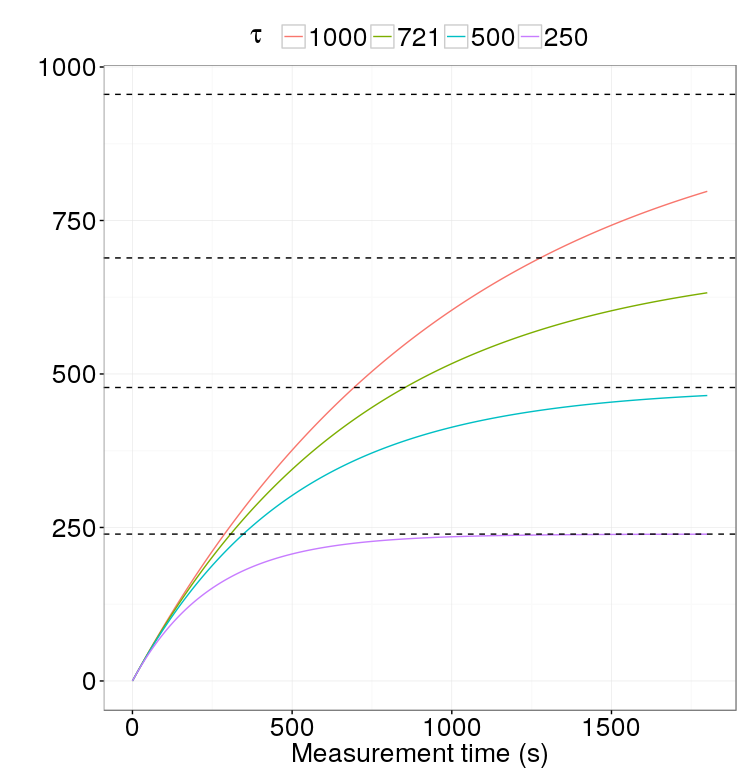
\includegraphics[scale=.5]{img/StatReq/XtotOnTime}
	\caption{$[g\circ t](\Nnd)$ for different life-times $\tau = \sfrac1\lambda$.\label{fig:GofT}}
\end{figure}
\begin{table}[h]
	\centering
	\caption{Total Fisher information, by what time it is reached,\\ and the corresponding signal-to-noise ratio.\label{tbl:FItot}}
	\begin{tabular}{rrr}
		\hline
		FI limit (\%) & Reached ($\times\tau$) & SNR \\ \hline
		           95 &                    3.0 & 1.0 \\
		           90 &                    2.3 & 1.9 \\
		           70 &                    1.2 & 4.7 \\
		           50 &                    0.7 & 7.1 \\ \hline
	\end{tabular}
\end{table}

Eq.~\eqref{eq:MeanFIZC},~\eqref{eq:NumMeasNode}, and
\[
	\stat* = \stat,
\]
produce an equation by which the required compaction time $\dtnd$ can be found:
\begin{equation}\label{eq:CmpTEq}
	\dtnd + \frac{\sin\omega\dtnd}{\omega} - 2\cdot \stat* \cdot\dtm \cdot g(\Nnd)^{-1}= 0.
\end{equation}

Assuming the polarimetry measurement time sufficient for 3\% error is 10$\mu$s, estimated compaction time (in percents of the signal quarter period --- 100\% is uniform sampling) is summarized in Table~\ref{tbl:CmpTvsSEw} and shown in Figure~\ref{fig:CmpTvsSEw}.

\begin{table}[h]
	\centering
	\caption{Compaction time.\label{tbl:CmpTvsSEw}}
	\begin{tabular}{rr}
		\hline
		$\SE{\hat{\omega}}$ (rad/sec) & $\dtnd$ (\%) \\ \hline
		$\vp{2}{-4}$ &        50.92 \\
		$\vp{5}{-4}$ &         7.74 \\
		$\vp{1}{-3}$ &         1.93 \\
		$\vp{2}{-3}$ &         0.48 \\
		$\vp{5}{-3}$ &         0.08 \\ \hline
	\end{tabular}
\end{table}

\begin{figure}[h]
	\centering
	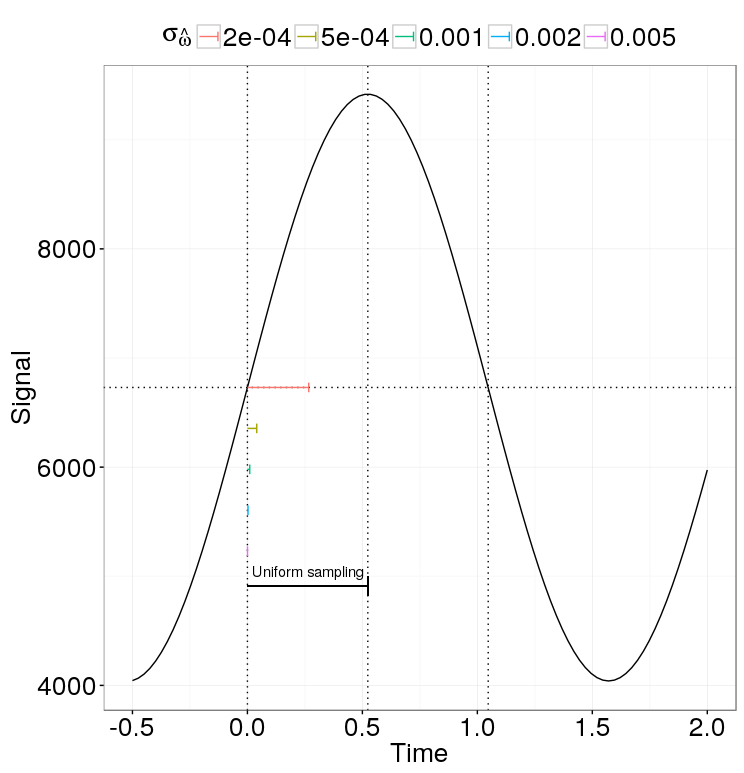
\includegraphics[scale=.5]{img/StatReq/CmpTvsSEw}
	\caption{Compaction time for different $\SE{\hat{\omega}}$.\label{fig:CmpTvsSEw}}
\end{figure}

\begin{figure}[h]
	\centering
	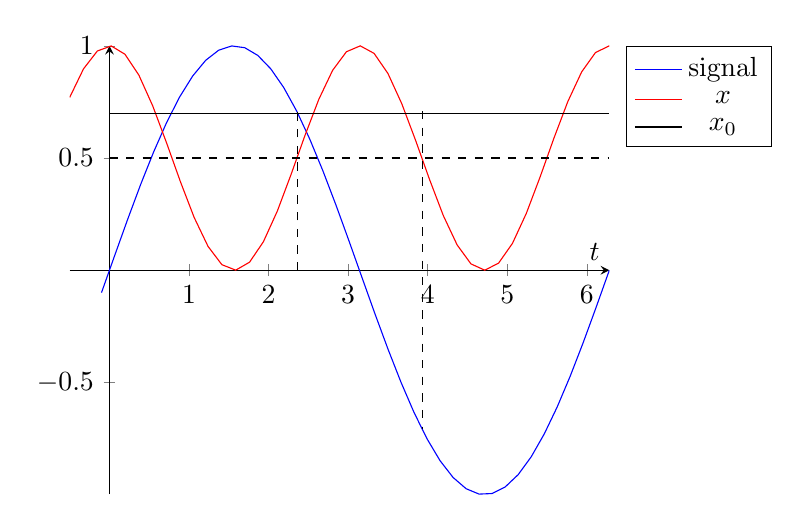
\begin{tikzpicture}
	\begin{axis}[axis lines=center, xlabel=$t$, domain=-.5:2*pi, legend pos=outer north east, samples=40]
	\addplot[color=blue, name path=signal, domain=-.1:2*pi] {sin(deg(x))}; \addlegendentry{signal}
	\addplot[color=red] {cos(deg(x))^2}; \addlegendentry{$x$}
	\addplot[mark=none, domain=0:2*pi]{.7}; \addlegendentry{$x_0$}
	\addplot[mark=none,dashed, domain=0:2*pi]{.5};
	\draw[dashed] (axis cs:2.36,0) -- (axis cs:2.36,{sin(deg(2.36))});
	\draw[dashed] (axis cs:3.93,{-sin(deg(3.93))}) -- (axis cs:3.93,{sin(deg(3.93))});
	\end{axis}
	\end{tikzpicture}
	\caption{Explanation for $x_0$\label{fig:x0Expl}.}
\end{figure}

\section{Time spread}

From Table~\ref{tbl:FItot} it follows that by the time $3\cdot \tau$ we'll exhaust most of the information contained in the beam, so that measuring afterward does not make sense. The quantity $\tau = \LTd/(1+x)$, where $x=\sfrac{\LTd}{\LTb}$, and it is less than either $\LTd$ or $\LTb$. We would, however, like to have our sample as spread out in time as possible, which means $\tau$ needs to be increased.

One way in which it is possible to do is by employing a non-uniform sampling scheme. This is beneficial in two respects:
\begin{inparaenum}[1)]
	\item in the first place, since we don't scatter the beam continuously, its life-time extends, thus extending the possible time-spread.
	\item in the second place, the particles preserved during the periods in which the absolute value of the signal's time derivative is lowest can be more advantageously used when the derivative is maximal.
\end{inparaenum} 

This means by modulating the sampling time, we can simultaneously increase both $\stat*$ and $\var[w]{t}$.

\section{Analysis}

In order to achieve a precision on the order of $10^{-29}~e\cdot cm$ in the dEDM estimate, it is required that the spin tune be known down to $10^{-9}~rad/sec$. 

For analysis, we will assume the following model of the signal:
\begin{equation}
	N(t) = pN_0^b\cdot\frac{\dtc}{\nu}\cdot\bkt{e^{\lamb\cdot t} + P\cdot e^{\lambda\cdot t}\cdot\sin(\omega\cdot t + \phi)}, ~ \lambda = (1+\sfrac{\LTd}{\LTb})\cdot \lamd.
\end{equation}
The parameters used in simulation are summarized in Table~\ref{tbl:ModParam}; the signal is plotted in Figure~\ref{fig:SignalModel}.
\begin{table}[h]
	\centering
	\caption{Model parameters.\label{tbl:ModParam}}
	\begin{tabular}{p{2.5cm}crr}
		\hline
		Parameter                 &      Symbol      & Value & Dimension \\ \hline
		Decoherence life-time     &      $\LTd$      &   721 &       sec \\
		Beam life-time            &      $\LTb$      &   721 &       sec \\
		Event error               & $\SD{\meas}/N_0$ &     3 &        \% \\
		Spin tune                 &     $\omega$     &     3 &   rad/sec \\
		Initial phase             &      $\phi$      &     0 &       rad \\
		Polarization              &       $P$        &   0.4 &      unit \\
		Unpolarized counting rate &     $N_0(0)$     &  6750 & count/sec \\ \hline
	\end{tabular}
\end{table}

\begin{figure}[h]
	\centering
	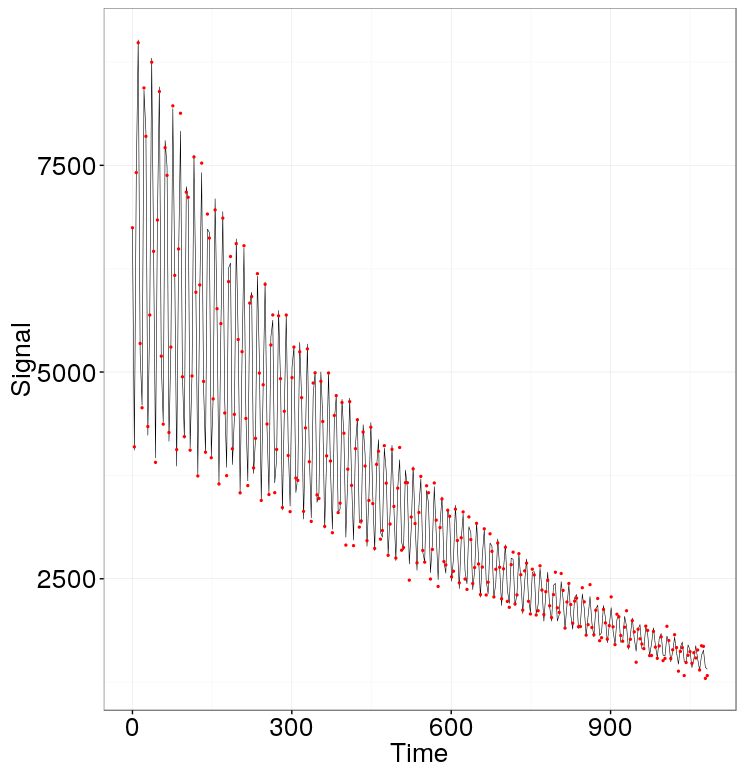
\includegraphics[scale=.8]{img/StatReq/Signal_model}
	\caption{Signal model.\label{fig:SignalModel}}
\end{figure}

For the given parameters, Figure~\ref{fig:SEw_vs_w} shows the lack of dependence of the standard error of the frequency estimate on the value of the estimated frequency.

The standard error of $2\cdot 10^{-7}$ is sufficiently low for the average estimate to be known with precision $10^{-9}$ rad/sec.

\begin{figure}[h]
	\centering
	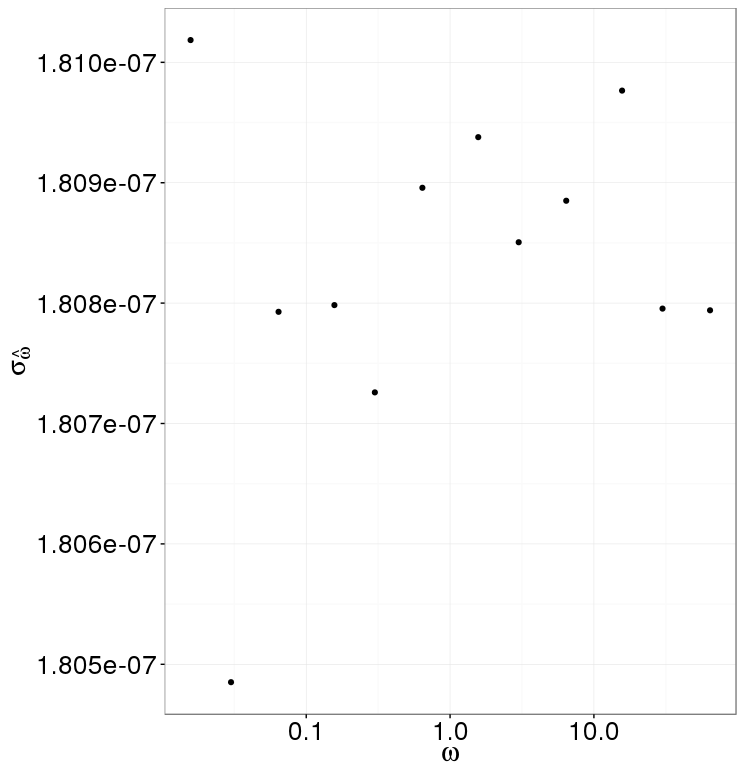
\includegraphics[scale=.8]{img/StatReq/SEw_vs_w}
	\caption{The standard error of the frequency estimate is independent of the estimated value.\label{fig:SEw_vs_w}}
\end{figure}

\begin{thebibliography}{9}
	\bibitem{CountRateStat}
	\url{http://www.owlnet.rice.edu/~dodds/Files331/stat_notes.pdf}.
\end{thebibliography}

\end{document}